\chapter{Shortest paths}
\label{ch:paths}

A mowing path is mostly straight passes. Between them, and every time the
mower moves from one region to another, it must go from one pose to another:
from the end of a pass, heading east, to the start of the next one, heading
west, a metre away. This chapter answers the question: what is the shortest
path between two poses for a vehicle whose curvature is limited, first when
it can only drive forward, then when it can also reverse?

\section{The problem, and how to simplify it}

\begin{definition}{Feasible path}{feasible}
  A \emph{feasible path} from the pose $q_0$ to the pose $q_1$ is a path of
  the middle of the rear axle that starts at $q_0$, ends at $q_1$, and
  satisfies the bicycle model (Theorem~\ref{thm:bicycle}) with
  $|\kappa| \le \kmax = 1/\Rmin$ at every point. Its \emph{length} counts
  forward and reverse distances alike. A point where the direction of travel
  changes is a \emph{cusp}.
\end{definition}

\begin{proposition}{Normalisation}{normalise}
  Let $q_0 = (x_0, y_0, \theta_0)$ and $q_1 = (x_1, y_1, \theta_1)$, and
  \begin{align*}
    x' &= \frac{\cos\theta_0\,(x_1 - x_0) + \sin\theta_0\,(y_1 - y_0)}{R},
    \\
    y' &= \frac{-\sin\theta_0\,(x_1 - x_0) + \cos\theta_0\,(y_1 - y_0)}{R},
    \\
    \varphi &= \theta_1 - \theta_0 .
  \end{align*}
  The feasible paths from $q_0$ to $q_1$ with curvature at most $1/R$
  correspond one to one to the feasible paths from $(0, 0, 0)$ to
  $(x', y', \varphi)$ with curvature at most $1$, and their lengths are in
  the ratio $R$.
\end{proposition}

\begin{proof}
  Moving the plane so that $q_0$ goes to the origin with heading $0$ is a
  rotation by $-\theta_0$ after a translation; it preserves lengths and
  curvatures, and takes $q_1$ to $(R x', R y', \varphi)$. Then scaling the
  plane by $1/R$ divides all lengths by $R$ and multiplies all curvatures by
  $R$, so $|\kappa| \le 1/R$ becomes $|\kappa| \le 1$. Both maps can be
  undone, hence the one-to-one correspondence.
\end{proof}

From now on the start is $(0, 0, 0)$ and the turning radius is $1$: an arc
of length $t$ turns the heading by $t$ radians. A path made of arcs of
maximal curvature and straight lines is written as a \emph{word}: L for an
arc to the left, R to the right, S for a straight line, each with a signed
length (negative in reverse). For example $L^+ S^+ L^+$ is ``left arc
forward, straight line forward, left arc forward''.

\section{Forward only: Dubins paths}

\begin{theorem}{Dubins, 1957}{dubins}
  Between any two poses, a shortest feasible path that only drives forward
  exists, and it is one of the six words
  \[
    LSL,\quad RSR,\quad LSR,\quad RSL \quad (\text{type } CSC),
    \qquad RLR,\quad LRL \quad (\text{type } CCC),
  \]
  where each arc has the maximal curvature, and in a $CCC$ word the middle
  arc is longer than $\pi$.
\end{theorem}

The proof~\cite{dubins1957curves} is
beyond this course; the theorem turns an optimisation over all paths into a
choice among six candidates, each given by a closed formula. The idea of the
$CSC$ formulas is plain geometry: the first arc runs on one of the two
circles tangent to the start pose, the last on one of the two circles tangent
to the goal, and the straight line is a common tangent of these circles.

\begin{proposition}{The word $LSL$}{lsl}
  Let $c_0 = (0, 1)$ be the centre of the left circle of the start pose and
  $c_1 = (x - \sin\varphi,\; y + \cos\varphi)$ the centre of the left circle
  of the goal $(x, y, \varphi)$. Write $c_1 - c_0 = u\,(\cos\alpha,
  \sin\alpha)$ with $u \ge 0$. Then $L^+ S^+ L^+$ with lengths
  \[
    t = \alpha \bmod 2\pi, \qquad u = |c_1 - c_0|, \qquad
    v = (\varphi - \alpha) \bmod 2\pi
  \]
  drives from $(0, 0, 0)$ to $(x, y, \varphi)$.
\end{proposition}

\begin{proof}
  A left arc of radius 1 starting at the pose $(p, \theta)$ runs on the
  circle of centre $p + n = p + (-\sin\theta, \cos\theta)$ (the centre of
  rotation, Proposition~\ref{prop:icr}). For the start, that is $c_0 = (0,
  1)$. For the goal, the last arc ends at $(x, y)$ with heading $\varphi$, so
  it runs on the circle of centre $c_1 = (x - \sin\varphi, y + \cos\varphi)$.

  On a left circle, a point and its heading are related by $p = c - n$: the
  car is on the right of the centre as seen in its direction of travel. The
  straight line leaves the first circle and joins the second with the same
  heading $\alpha$ (it is a straight line), at the points
  $c_0 - n_\alpha$ and $c_1 - n_\alpha$, with $n_\alpha = (-\sin\alpha,
  \cos\alpha)$. The segment between them is $c_1 - c_0$, which must point
  along $(\cos\alpha, \sin\alpha)$: this is the definition of $\alpha$, and
  the length of the segment is $u = |c_1 - c_0|$. The first arc turns the
  heading from $0$ to $\alpha$, an arc of length $t = \alpha \bmod 2\pi$;
  the last turns it from $\alpha$ to $\varphi$, an arc of length $(\varphi -
  \alpha) \bmod 2\pi$.
\end{proof}

\begin{figure}[ht]
  \centering
  \begin{tikzpicture}[scale=1.25, >=Stealth, font=\small]
    \def\a{17.697}
    \coordinate (c0) at (0,1);
    \coordinate (c1) at (3.134,2);
    \draw[black!40] (c0) circle (1);
    \draw[black!40] (c1) circle (1);
    \fill (c0) circle (0.04) node[left] {$c_0$};
    \fill (c1) circle (0.04) node[above right] {$c_1$};
    \draw[densely dotted] (c0) -- (c1) node[pos=0.55, above] {$u$};
    % tangent points: c - n_alpha
    \coordinate (T0) at ($(c0)+({sin(\a)},{-cos(\a)})$);
    \coordinate (T1) at ($(c1)+({sin(\a)},{-cos(\a)})$);
    \draw[very thick, blue!70!black] (0,0) arc[start angle=-90,
      end angle={-90+\a}, radius=1];
    \draw[very thick, blue!70!black] (T0) -- (T1);
    \draw[very thick, blue!70!black] (T1) arc[start angle={-90+\a},
      end angle={-90+60}, radius=1];
    % start and goal poses
    \draw[->, very thick, green!50!black] (0,0) -- (0.7,0);
    \node[below] at (0,0) {start $(0,0,0)$};
    \coordinate (G) at (4,1.5);
    \draw[->, very thick, violet] (G) -- ++(60:0.7);
    \node[right] at (G) {goal $(4, 1.5, 60°)$};
    \coordinate (O) at (0,0);
    \draw[dashed] (c0) -- (O);
    \draw[dashed] (c0) -- (T0);
    \pic[draw, "$t$", angle radius=0.55cm, angle eccentricity=1.35]
      {angle=O--c0--T0};
  \end{tikzpicture}
  \caption{The construction of an $L^+S^+L^+$ path (normalised, turning
    radius 1) from $(0, 0, 0)$ to $(4, 1.5, 60°)$. The first arc runs on the
    left circle of the start (centre $c_0$), the last on the left circle of
    the goal (centre $c_1$), and the straight line, parallel to $c_1 - c_0$,
    is tangent to both. Here $u = 3.290$, $t = 0.309$ ($17.7°$) and
    $v = 0.738$ ($42.3°$), for a total length of $4.337$; it is the
    shortest of the five Dubins words that exist for this goal.}
  \label{fig:lsl}
\end{figure}

\begin{example}{$LSL$ to $(4, 1.5, 60°)$}{lslnum}
  With $\varphi = 60°$: $c_1 = (4 - \sin 60°,\; 1.5 + \cos 60°) = (4 -
  0.8660,\; 1.5 + 0.5) = (3.1340, 2.0)$, so $c_1 - c_0 = (3.1340, 1.0)$ and
  \begin{align*}
    u &= \sqrt{3.1340^2 + 1.0^2} = 3.2897, \qquad
    \alpha = \atantwo(1.0, 3.1340) = \SI{0.3089}{\radian}\;(17.7°), \\
    t &= 0.3089, \qquad v = \varphi - \alpha = 1.0472 - 0.3089
      = \SI{0.7383}{\radian}\;(42.3°),
  \end{align*}
  a total length of $0.3089 + 3.2897 + 0.7383 = 4.3369$ times the turning
  radius (Figure~\ref{fig:lsl}).
\end{example}

The other five words have formulas of the same kind (the code lists them in
\code{dubins\_words}). The code computes all six, keeps those that exist and
really reach the goal, and returns the shortest.

\section{With reverse: Reeds--Shepp paths}

\begin{theorem}{Reeds and Shepp, 1990~\cite{reeds1990optimal}}{reedsshepp}
  If the vehicle may also reverse, a shortest feasible path between two poses
  is one of 48 words of at most five segments, with at most two cusps. Up to
  the symmetries below, they form nine families, written with ``$|$'' at a
  cusp:
  \begin{gather*}
    C|C|C,\qquad CC|C,\qquad C|CC,\qquad CSC,\qquad CC_u|C_uC,\\
    C|C_uC_u|C,\qquad C|C_{\pi/2}SC,\qquad CSC_{\pi/2}|C,\qquad
    C|C_{\pi/2}SC_{\pi/2}|C,
  \end{gather*}
  where $C_u$ denotes two arcs of the same length $u$ and $C_{\pi/2}$ an arc
  of a quarter turn.
\end{theorem}

The 48 words do not need 48 formulas. Two symmetries map solutions onto
solutions:

\begin{proposition}{Time flip and reflection}{symmetries}
  Suppose a word, with letters $X_1 \dots X_k$ and signed lengths $s_1, \dots,
  s_k$, drives from $(0, 0, 0)$ to $(x, y, \varphi)$. Then
  \begin{enumerate}
    \item \emph{time flip}: the same letters with lengths $-s_1, \dots,
      -s_k$ drive from $(0, 0, 0)$ to $(-x, y, -\varphi)$;
    \item \emph{reflection}: the lengths $s_1, \dots, s_k$ with every L
      changed into R and every R into L drive from $(0, 0, 0)$ to
      $(x, -y, -\varphi)$.
  \end{enumerate}
\end{proposition}

\begin{proof}
  Along the path, the pose $(x(s), y(s), \theta(s))$ satisfies
  $d\theta/ds = \kappa$, $dx/ds = \cos\theta$, $dy/ds = \sin\theta$.

  \emph{Time flip.} Let $\tilde s = -s$ and $(\tilde x, \tilde y,
  \tilde\theta) = (-x, y, -\theta)$. Then
  \[
    \frac{d\tilde\theta}{d\tilde s} = \frac{d\theta}{ds} = \kappa, \quad
    \frac{d\tilde x}{d\tilde s} = \frac{dx}{ds} = \cos\theta
      = \cos\tilde\theta, \quad
    \frac{d\tilde y}{d\tilde s} = -\frac{dy}{ds} = -\sin\theta
      = \sin\tilde\theta,
  \]
  so the new pose follows the bicycle model with the same curvature (the
  same letters), along signed lengths of opposite signs. It starts at
  $(0, 0, 0)$ and ends at $(-x, y, -\varphi)$.

  \emph{Reflection.} Let $(\tilde x, \tilde y, \tilde\theta) = (x, -y,
  -\theta)$ with the same $s$. Then $d\tilde\theta/ds = -\kappa$ (L and R
  swap), $d\tilde x/ds = \cos\theta = \cos\tilde\theta$ and $d\tilde y/ds =
  -\sin\theta = \sin\tilde\theta$. It ends at $(x, -y, -\varphi)$.
\end{proof}

So to find the words of a given type reaching $(x, y, \varphi)$, it is enough
to have one formula, and to apply it to the four goals $(x, y, \varphi)$,
$(-x, y, -\varphi)$, $(x, -y, -\varphi)$ and $(-x, -y, \varphi)$, then flip,
reflect, or both, the solutions found. Twelve base formulas, applied four
times each, give the 48 words.

\paragraph{How the code makes sure every word is right.}
The closed formulas are easy to get subtly wrong. The code therefore never
trusts a formula alone: each candidate word is driven with the exact arc
formulas of Proposition~\ref{prop:arc}, and kept only if it ends at the goal
(within $10^{-5}$). The tests then check, on thousands of random pairs of
poses, that all 48 words occur, that the distance found is symmetric
(as short from $q_0$ to $q_1$ as back) and satisfies the triangle
inequality, that it is never longer than the result of an independent
implementation, and that whenever the shortest Reeds--Shepp path happens to
drive only forward, it has exactly the length of the shortest Dubins path.
Both families, with the geometric arguments behind them, are presented in
Section~15.3 of LaValle's \emph{Planning Algorithms}~\cite{lavalle2006planning}.

\begin{figure}[ht]
  \centering
  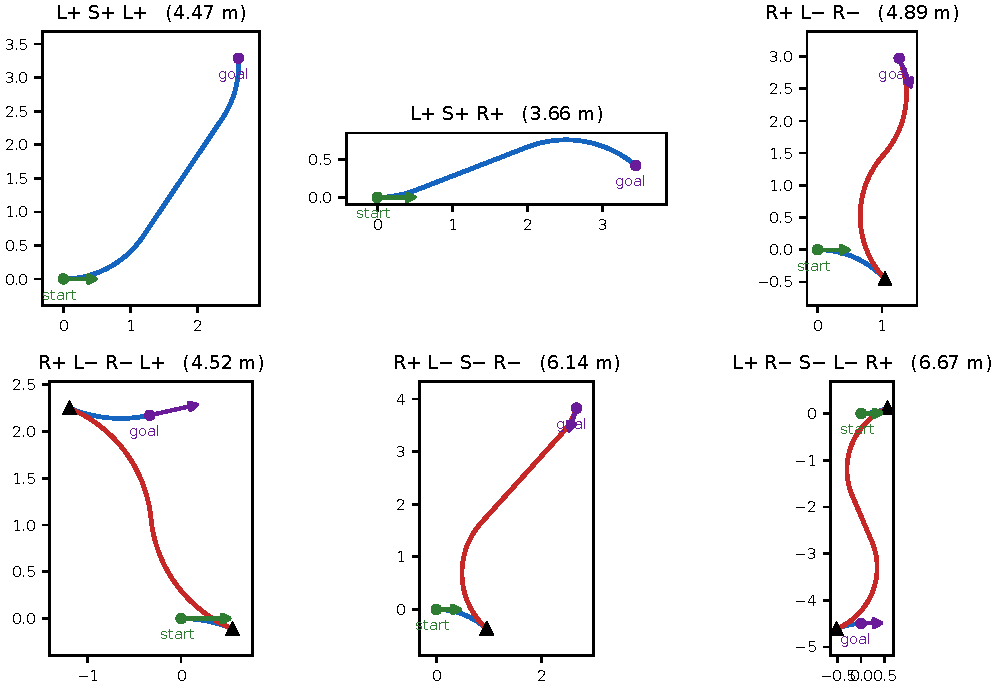
\includegraphics[width=\textwidth]{figures/rs_examples}
  \caption{Shortest Reeds--Shepp paths from the pose $(0, 0, 0)$ (green
    arrow) to six other poses (purple arrows), for the default mower
    (turning radius \SI{1.43}{\metre}, axes in metres). Blue: forward, red:
    reverse; black triangles: cusps. The word above each panel gives each
    segment's letter and direction ($+$ forward, $-$ reverse).}
  \label{fig:rsexamples}
\end{figure}

\section{The mowing case: turning into the next pass}
\label{sec:nextpass}

Every back-and-forth pattern meets the same manoeuvre: at the end of a pass
heading east, go to the start of the next pass, one cutting width over
(minus a small overlap), heading west. For the default mower this is the goal
$(0, \SI{0.92}{\metre}, 180°)$ from $(0, 0, 0)$, with
$\Rmin = \SI{1.4301}{\metre}$; in normalised coordinates,
$(0,\; 0.92 / 1.4301,\; \pi) = (0, 0.6433, \pi)$.

The difficulty is that the next pass is closer than $2\Rmin =
\SI{2.86}{\metre}$, the sideways shift of a half-turn at full lock. Driving
forward only, the mower cannot simply turn round: it must first swing away
from the next pass, then loop back (a ``bulb'' turn). With reverse, it can
make a three-point turn instead.

\begin{figure}[ht]
  \centering
  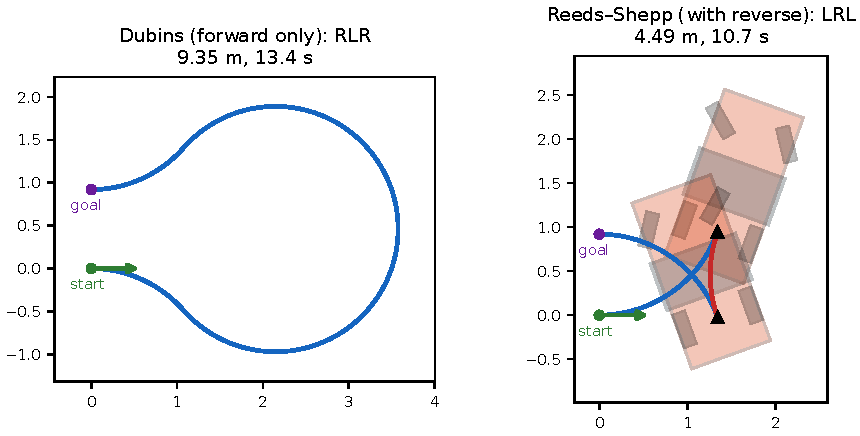
\includegraphics[width=\textwidth]{figures/next_pass}
  \caption{Going from the end of a pass (green arrow, heading east) to the
    start of the next one, \SI{0.92}{\metre} to the left (purple arrow,
    heading west), for the default mower. Left: the shortest forward-only
    path, a bulb turn $RLR$ of \SI{9.35}{\metre}. Right: the shortest path
    with reverse, a three-point turn $L^+R^-L^+$ of \SI{4.49}{\metre}; the
    mower is drawn at its two cusps (black triangles). Blue: forward, red:
    reverse. Times use the speeds of Table~\ref{tab:speeds}.}
  \label{fig:nextpass}
\end{figure}

The shortest path is not the end of the story. Changing direction means
stopping, changing gear and starting again, and reversing is slower. The code
estimates the time of a path with a simple model:

\begin{definition}{Time of a path}{time}
  With $v_{\mathrm{mow}}$ the forward speed on straight lines,
  $v_{\mathrm{turn}}$ the forward speed on arcs, $v_{\mathrm{rev}}$ the
  reverse speed and $t_{\mathrm{shift}}$ the time lost at each cusp,
  \[
    t = \sum_{\text{straight, forward}} \frac{\ell_i}{v_{\mathrm{mow}}}
      + \sum_{\text{arc, forward}} \frac{\ell_i}{v_{\mathrm{turn}}}
      + \sum_{\text{reverse}} \frac{\ell_i}{v_{\mathrm{rev}}}
      + n_{\mathrm{cusps}}\, t_{\mathrm{shift}} .
  \]
\end{definition}

\begin{table}[ht]
  \centering
  \begin{tabular}{@{}lr@{}}
    \toprule
    forward speed on straight lines, $v_{\mathrm{mow}}$ &
      \SI{1.2}{\metre\per\second} \\
    forward speed on arcs, $v_{\mathrm{turn}}$ & \SI{0.7}{\metre\per\second} \\
    reverse speed, $v_{\mathrm{rev}}$ & \SI{0.6}{\metre\per\second} \\
    time lost at each change of direction, $t_{\mathrm{shift}}$ &
      \SI{2}{\second} \\
    \bottomrule
  \end{tabular}
  \caption{Default speeds of the time model (parameters of the mower).}
  \label{tab:speeds}
\end{table}

\begin{example}{Bulb turn or three-point turn?}{threepoint}
  The bulb turn $R^+L^+R^+$ has arcs of \SI{1.2140}{\metre},
  \SI{6.9208}{\metre} and \SI{1.2140}{\metre}, all forward on arcs:
  \[
    t = \frac{1.2140 + 6.9208 + 1.2140}{0.7} = \frac{9.3488}{0.7}
    = \SI{13.36}{\second}.
  \]
  The three-point turn $L^+R^-L^+$ has two forward arcs of
  \SI{1.7515}{\metre}, a reverse arc of \SI{0.9897}{\metre} and two cusps:
  \[
    t = \frac{1.7515 + 1.7515}{0.7} + \frac{0.9897}{0.6} + 2 \times 2
    = 5.004 + 1.650 + 4 = \SI{10.65}{\second}.
  \]
  Even with two stops, the three-point turn is faster, and it needs much
  less room: in the bulb turn, the rear axle goes \SI{3.6}{\metre} beyond
  the end of the pass, against \SI{1.3}{\metre} in the three-point turn.
\end{example}

\begin{figure}[ht]
  \centering
  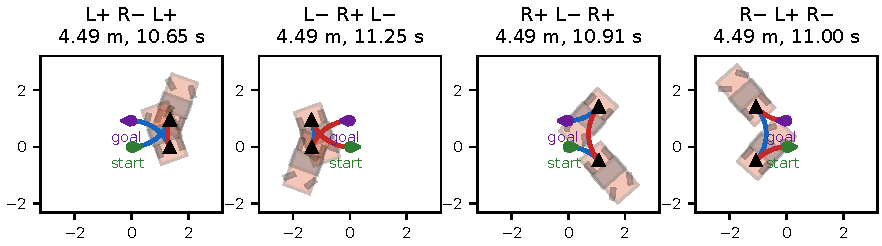
\includegraphics[width=\textwidth]{figures/ties}
  \caption{The four shortest Reeds--Shepp paths for the turn of
    Figure~\ref{fig:nextpass}: all are \SI{4.49}{\metre} long, but they take
    different times, because they reverse over different distances. Above
    each panel: the word, its length and its time with the speeds of
    Table~\ref{tab:speeds}.}
  \label{fig:ties}
\end{figure}

For this turn there are four shortest paths (Figure~\ref{fig:ties}), with the
same length but different times. This is why the code has two functions:
\code{shortest} returns a shortest path, and \code{fastest} returns, among
all the Reeds--Shepp candidates, the one with the least time. The latter is
not a time-optimal planner (the fastest path might be none of the
candidates), but it is the right choice among them.

\begin{inwords}
  For a car-like mower, the closest next strip is the hardest to reach: it
  is nearer than twice the turning radius. Reverse turns a long loop into a
  short three-point turn, and is worth its stops. The same pose-to-pose
  problem appears everywhere a planner joins two pieces of path, so these
  formulas are the bricks of all later chapters.
\end{inwords}

\begin{incode}
  \code{mowersim/paths.py}: \code{normalise} (Proposition~\ref{prop:normalise}),
  \code{dubins\_words}, the twelve Reeds--Shepp base formulas and
  \code{reeds\_shepp\_words} (Proposition~\ref{prop:symmetries}),
  \code{candidates} (each word is driven to check it reaches the goal),
  \code{shortest}, \code{fastest} and \code{path\_time}
  (Definition~\ref{def:time}). \code{python -m mowersim path 0 0.92 180
  -{}-compare} prints Example~\ref{ex:threepoint}.
\end{incode}
